In conclusione il grafico in Figura (5) rispetta le previsioni teoriche: l'angolo di incidenza $\delta$ decresce, raggiunge un valore minimo e poi torna a crescere, al crescere dell'angolo di incidenza $\theta_i$. Coi dati raccolti, è inoltre possibile confrontare lo stesso grafico con la curva teorica descritta dalla Legge (10).

\begin{figure}[H]
	\centering
	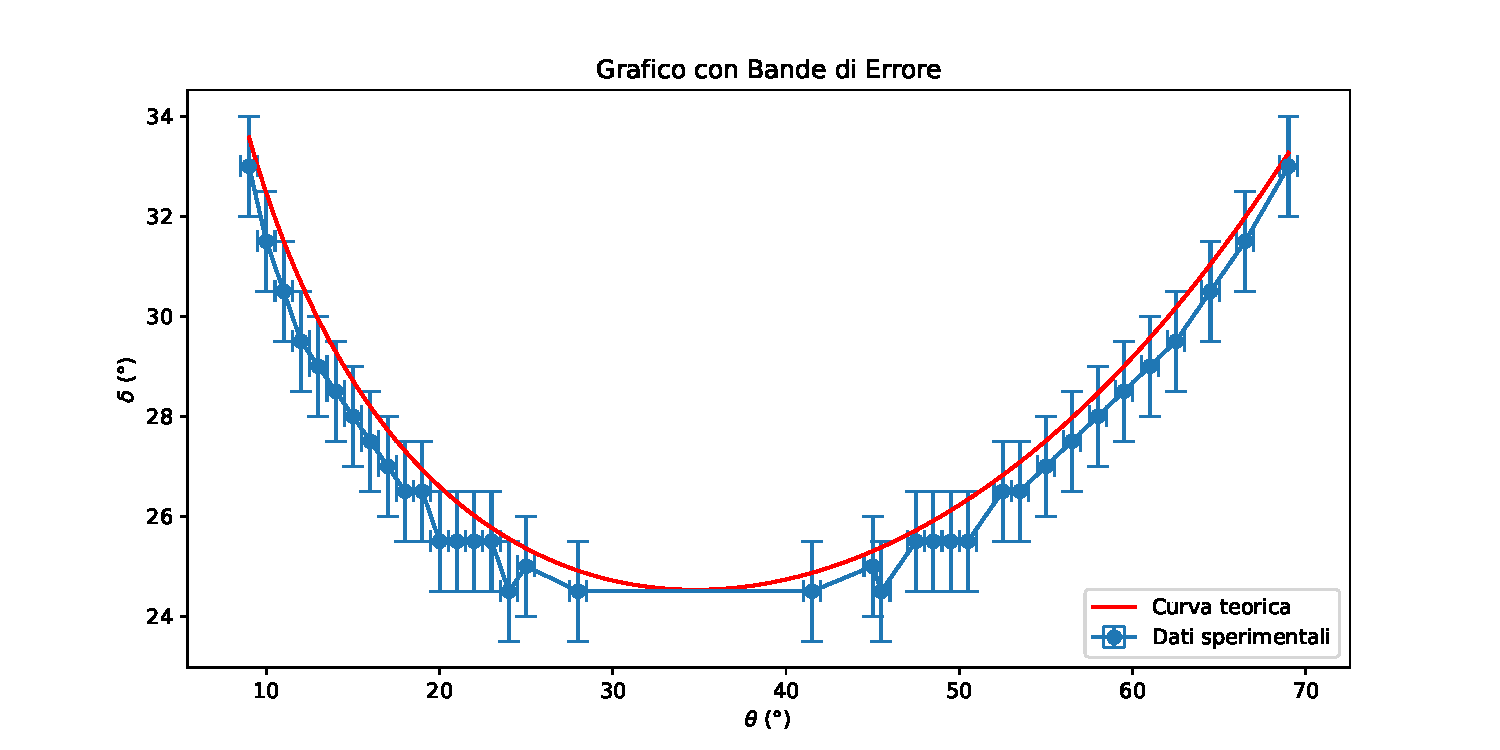
\includegraphics[width=0.95\textwidth]{./figures/grafico2.pdf}
	\captionsetup{width=0.7\linewidth}
	\caption{I dati sperimentali ottenuti mostrano un buon accordo con l'andamento teorico previsto. La curva teorica si interpola infatti all'interno dell'intervallo di incertezza associato ai dati sperimentali. Eventuali discrepanze residue possono essere attribuite a errori sperimentali sistematici o a imprecisioni nella misura degli angoli.}
\end{figure}